% ═══════════════════════════════════════════════════════════════
%  Modern Light Presentation — RL Snake
%  Compile: pdflatex presentation.tex (2 passes)
% ═══════════════════════════════════════════════════════════════
\documentclass[aspectratio=169]{beamer}

\PassOptionsToPackage{table}{xcolor}
\usepackage[T2A]{fontenc}
\usepackage[utf8]{inputenc}
\usepackage[main=russian,english]{babel}
\usepackage{graphicx}
\usepackage{booktabs}
\usepackage{tabularx}
\usepackage{amsmath}
\usepackage{tikz}
\usepackage{colortbl}
\usepackage{lmodern}
\usepackage{microtype}
\usepackage{calc}

\usetikzlibrary{
  shapes.geometric,
  positioning,
  calc,
  arrows.meta,
  shadows.blur,
  decorations.pathreplacing
}

\graphicspath{{../overleaf-sync/images/}}

% ── Color Palette (refined, warm-slate) ─────────────────────
\definecolor{accent}{HTML}{3B82F6}        % blue-500
\definecolor{accentdark}{HTML}{1D4ED8}     % blue-700
\definecolor{accentlight}{HTML}{EFF6FF}    % blue-50
\definecolor{accentmid}{HTML}{93C5FD}      % blue-300
\definecolor{textmain}{HTML}{0F172A}       % slate-900
\definecolor{textsub}{HTML}{64748B}        % slate-500
\definecolor{textweak}{HTML}{94A3B8}       % slate-400
\definecolor{surfacebg}{HTML}{FFFFFF}
\definecolor{surfacecard}{HTML}{F1F5F9}    % slate-100
\definecolor{ruleclr}{HTML}{CBD5E1}        % slate-300
\definecolor{greenclr}{HTML}{22C55E}       % green-500
\definecolor{greenbg}{HTML}{F0FDF4}        % green-50
\definecolor{redclr}{HTML}{EF4444}         % red-500
\definecolor{redbg}{HTML}{FEF2F2}          % red-50
\definecolor{amberclr}{HTML}{F59E0B}       % amber-500
\definecolor{amberbg}{HTML}{FFFBEB}        % amber-50

% ── Beamer Theme (minimal) ──────────────────────────────────
\usetheme{default}
\setbeamercolor{background canvas}{bg=surfacebg}
\setbeamercolor{normal text}{fg=textmain}
\setbeamercolor{frametitle}{fg=textmain}
\setbeamercolor{structure}{fg=accent}
\setbeamercolor{itemize item}{fg=accent}
\setbeamercolor{alerted text}{fg=redclr}

\setbeamertemplate{navigation symbols}{}
\setbeamertemplate{headline}{}

\setbeamerfont{frametitle}{size=\Large,series=\bfseries}
\setbeamerfont{title}{size=\LARGE,series=\bfseries}
\setbeamerfont{subtitle}{size=\normalsize,series=\mdseries}
\setbeamerfont{author}{size=\normalsize}
\setbeamerfont{institute}{size=\small}
\setbeamerfont{date}{size=\small}

% ── Custom Bullet ───────────────────────────────────────────
\setbeamertemplate{itemize item}{%
  \tikz[baseline=-0.6ex]{\fill[accent] (0,0) circle(1.5pt);}}
\setbeamertemplate{itemize subitem}{%
  \tikz[baseline=-0.6ex]{\fill[accentmid] (0,0) circle(1.2pt);}}

% ── Custom Frame Title ──────────────────────────────────────
\setbeamertemplate{frametitle}{%
  \vskip6pt%
  \usebeamerfont{frametitle}\usebeamercolor[fg]{frametitle}\insertframetitle%
  \ifx\insertframesubtitle\empty\else%
    \\[1pt]{\usebeamerfont{framesubtitle}\textcolor{textsub}{\insertframesubtitle}}%
  \fi%
  \vskip4pt%
  \begin{tikzpicture}
    \fill[accent] (0,0) rectangle (2.4cm,2pt);
    \fill[ruleclr] (2.4cm,0) rectangle (\textwidth,0.6pt);
  \end{tikzpicture}%
  \vskip2pt%
}

% ── Footer: progress bar + slide number ─────────────────────
\setbeamertemplate{footline}{%
  \begin{tikzpicture}[remember picture,overlay]
    \fill[ruleclr] (current page.south west) rectangle
      ([yshift=3pt]current page.south east);
    \fill[accent] (current page.south west) rectangle
      ([yshift=3pt,xshift=\dimexpr\paperwidth*\insertframenumber/\inserttotalframenumber]current page.south west);
    \node[anchor=south east,font=\scriptsize,text=textweak]
      at ([xshift=-8pt,yshift=6pt]current page.south east)
      {\insertframenumber\,/\,\inserttotalframenumber};
  \end{tikzpicture}%
}

% ── Helper commands ─────────────────────────────────────────
\newcommand{\tagbox}[3]{% color-bg, color-fg, text
  \tikz[baseline=(T.base)]{%
    \node[fill=#1, rounded corners=4pt, inner xsep=5pt, inner ysep=3pt,
          font=\small\bfseries, text=#2](T){#3};}%
}
\newcommand{\accenttag}[1]{\tagbox{accentlight}{accentdark}{#1}}
\newcommand{\greentag}[1]{\tagbox{greenbg}{greenclr!80!black}{#1}}
\newcommand{\redtag}[1]{\tagbox{redbg}{redclr!80!black}{#1}}
\newcommand{\ambertag}[1]{\tagbox{amberbg}{amberclr!80!black}{#1}}

\newcommand{\cardbox}[2]{% width, content
  \begin{tikzpicture}
    \node[draw=ruleclr, fill=surfacecard, rounded corners=8pt,
          blur shadow={shadow blur steps=5,shadow xshift=0.5pt,
                       shadow yshift=-1pt,shadow blur radius=2pt},
          inner sep=12pt, text width=#1, align=left](C){#2};
  \end{tikzpicture}%
}

\newcommand{\cardboxc}[2]{% centered card
  \begin{tikzpicture}
    \node[draw=ruleclr, fill=surfacecard, rounded corners=8pt,
          blur shadow={shadow blur steps=5,shadow xshift=0.5pt,
                       shadow yshift=-1pt,shadow blur radius=2pt},
          inner sep=12pt, text width=#1, align=center](C){#2};
  \end{tikzpicture}%
}

% ── Metadata ────────────────────────────────────────────────
\title{Обучение с подкреплением\\для игры <<Змейка>>}
\subtitle{Курсовая работа}
\author{Полегина~А.\,Д.}
\institute{БГУ, мехмат, каф.\ дифф.\ уравнений и системного анализа\\
           Научный руководитель: к.\,ф.-м.\,н., доцент С.\,Г.\,Красовский}
\date{Минск, 2026}

\begin{document}

% ═══════════════════════════════════════════════════════════════
%  SLIDE 1 — Title
% ═══════════════════════════════════════════════════════════════
\begin{frame}[plain]
\begin{tikzpicture}[remember picture,overlay]
  % Top decorative band
  \fill[accentlight]
    (current page.north west) rectangle
    ([yshift=-2.2cm]current page.north east);
  \fill[accent,opacity=0.8]
    ([yshift=-2.2cm]current page.north west) rectangle
    ([yshift=-2.4cm]current page.north east);
  % Bottom-right circle accent
  \fill[accent,opacity=0.06]
    ([xshift=-2cm,yshift=2cm]current page.south east) circle(4cm);
  \fill[accentmid,opacity=0.08]
    ([xshift=-4cm,yshift=1cm]current page.south east) circle(2.5cm);
\end{tikzpicture}

\vspace{-0.6cm}
\begin{tikzpicture}[remember picture,overlay]
  \node[anchor=north west,font=\footnotesize\bfseries,text=accent,
        inner sep=0pt]
    at ([xshift=1cm,yshift=-0.3cm]current page.north west)
    {БГУ\quad МЕХМАТ\quad 2026};
\end{tikzpicture}

\vspace{1.8cm}
\begin{flushleft}
\hspace{1cm}%
\begin{minipage}{0.78\textwidth}
  \usebeamerfont{title}\usebeamercolor[fg]{normal text}\inserttitle\\[8pt]
  \textcolor{accent}{\rule{3.5cm}{3pt}}\\[10pt]
  \usebeamerfont{subtitle}\textcolor{textsub}{\insertsubtitle}\\[12pt]
  \usebeamerfont{author}\insertauthor\\[4pt]
  \usebeamerfont{institute}\textcolor{textsub}{\insertinstitute}\\[6pt]
  \usebeamerfont{date}\textcolor{textsub}{\insertdate}
\end{minipage}
\end{flushleft}
\end{frame}

% ═══════════════════════════════════════════════════════════════
%  SLIDE 2 — Goal & Tasks
% ═══════════════════════════════════════════════════════════════
\begin{frame}{Цель и задачи}

\textbf{Цель:} разработать игру <<Змейка>> на Python, реализовать Q-learning для управления агентом и оценить качество обучения.

\vspace{0.5cm}
\begin{columns}[T]
\column{0.54\textwidth}
\textcolor{textsub}{\footnotesize ЗАДАЧИ}
\vspace{0.2cm}
\begin{itemize}\setlength\itemsep{0.25cm}
    \item Изучить алгоритм Q-learning
    \item Реализовать логику игры и RL-среду
    \item Задать состояние, действия и награду
    \item Провести эксперименты
\end{itemize}

\column{0.42\textwidth}
\cardbox{0.88\linewidth}{%
  \textcolor{textsub}{\footnotesize ПОЧЕМУ <<ЗМЕЙКА>> + RL}\\[8pt]
  \accenttag{Дискретная среда}\\[5pt]
  \accenttag{Мало действий}\\[5pt]
  \accenttag{Наглядный результат}%
}
\end{columns}
\end{frame}

% ═══════════════════════════════════════════════════════════════
%  SLIDE 3 — Approach Comparison
% ═══════════════════════════════════════════════════════════════
\begin{frame}{Сравнение подходов}

\centering
\renewcommand{\arraystretch}{1.4}
\begin{tabularx}{0.92\textwidth}{%
  >{\raggedright\arraybackslash}p{0.24\textwidth}
  >{\raggedright\arraybackslash}p{0.28\textwidth}
  >{\raggedright\arraybackslash}X}
    \arrayrulecolor{ruleclr}
    \toprule
    \textcolor{textsub}{\footnotesize Подход}
      & \textcolor{textsub}{\footnotesize Плюсы}
      & \textcolor{textsub}{\footnotesize Минусы} \\
    \midrule
    Правила и эвристики & Простота реализации & Слабая адаптивность \\
    Поиск траектории    & Явный маршрут       & Нет обучения на опыте \\
    \rowcolor{accentlight}
    \textcolor{accentdark}{\textbf{Табличный Q-learning}}
      & \textbf{Интерпретируемость}, связь с дискретной средой
      & Масштабируемость \\
    DQN                 & Сложные состояния   & Много ресурсов \\
    \bottomrule
\end{tabularx}
\renewcommand{\arraystretch}{1.0}

\vspace{0.4cm}
\accenttag{Выбран табличный Q-learning}\quad{\small--- баланс простоты и пользы}
\end{frame}

% ═══════════════════════════════════════════════════════════════
%  SLIDE 4 — State Vector
% ═══════════════════════════════════════════════════════════════
\begin{frame}{Состояние агента}
\framesubtitle{Вектор из 11 бинарных признаков}

\centering\vspace{0.1cm}
\begin{tikzpicture}[
    bar/.style={rounded corners=5pt, minimum width=9.8cm,
                minimum height=0.75cm, font=\normalsize,
                draw=none, text=white, align=center},
  ]
  \node[bar, fill=redclr!85!black]   (d) at (0,2.0)
    {danger\_straight\quad danger\_left\quad danger\_right};
  \node[bar, fill=accentdark!85]     (r) at (0,0.95)
    {dir\_up\quad dir\_down\quad dir\_left\quad dir\_right};
  \node[bar, fill=greenclr!70!black] (f) at (0,-0.1)
    {food\_left\quad food\_right\quad food\_up\quad food\_down};

  \node[font=\small\bfseries,text=redclr!80!black,anchor=east]
    at ([xshift=-0.3cm]d.west) {3};
  \node[font=\small\bfseries,text=accentdark,anchor=east]
    at ([xshift=-0.3cm]r.west) {4};
  \node[font=\small\bfseries,text=greenclr!70!black,anchor=east]
    at ([xshift=-0.3cm]f.west) {4};
\end{tikzpicture}

\vspace{0.35cm}
\begin{columns}[c]
\column{0.30\textwidth}\centering\redtag{Опасность рядом}
\column{0.30\textwidth}\centering\accenttag{Направление}
\column{0.30\textwidth}\centering\greentag{Положение пищи}
\end{columns}

\vspace{0.3cm}
{\small Компактное описание $\Rightarrow$ подходит для табличного Q-learning}
\end{frame}

% ═══════════════════════════════════════════════════════════════
%  SLIDE 5 — Actions & Reward
% ═══════════════════════════════════════════════════════════════
\begin{frame}{Действия и награда}

\begin{columns}[T]
\column{0.48\textwidth}
\textcolor{textsub}{\footnotesize 3 ОТНОСИТЕЛЬНЫХ ДЕЙСТВИЯ}
\vspace{0.2cm}

\centering
\accenttag{Прямо}\quad\accenttag{Влево}\quad\accenttag{Вправо}

\vspace{0.35cm}
\raggedright
{\small Относительные действия уменьшают избыточность: одинаковый смысл при любом направлении}

\column{0.48\textwidth}
\textcolor{textsub}{\footnotesize ФУНКЦИЯ НАГРАДЫ}
\vspace{0.2cm}

\centering
\renewcommand{\arraystretch}{1.4}
\begin{tabular}{@{}>{\centering}p{2.8cm}>{\centering\arraybackslash}p{2cm}@{}}
    \arrayrulecolor{ruleclr}
    \toprule
    \textcolor{textsub}{\footnotesize Событие} & \textcolor{textsub}{\footnotesize Награда} \\
    \midrule
    \greentag{Пища}       & $\boldsymbol{+10}$  \\[3pt]
    \redtag{Столкновение}  & $\boldsymbol{-10}$  \\[3pt]
    {\small Шаг}           & $-0.1$              \\
    \bottomrule
\end{tabular}
\renewcommand{\arraystretch}{1.0}

\vspace{0.25cm}
{\small Штраф за шаг $\Rightarrow$ агент не движется по кругу}
\end{columns}
\end{frame}

% ═══════════════════════════════════════════════════════════════
%  SLIDE 6 — Architecture
% ═══════════════════════════════════════════════════════════════
\begin{frame}{Архитектура программной системы}
\centering
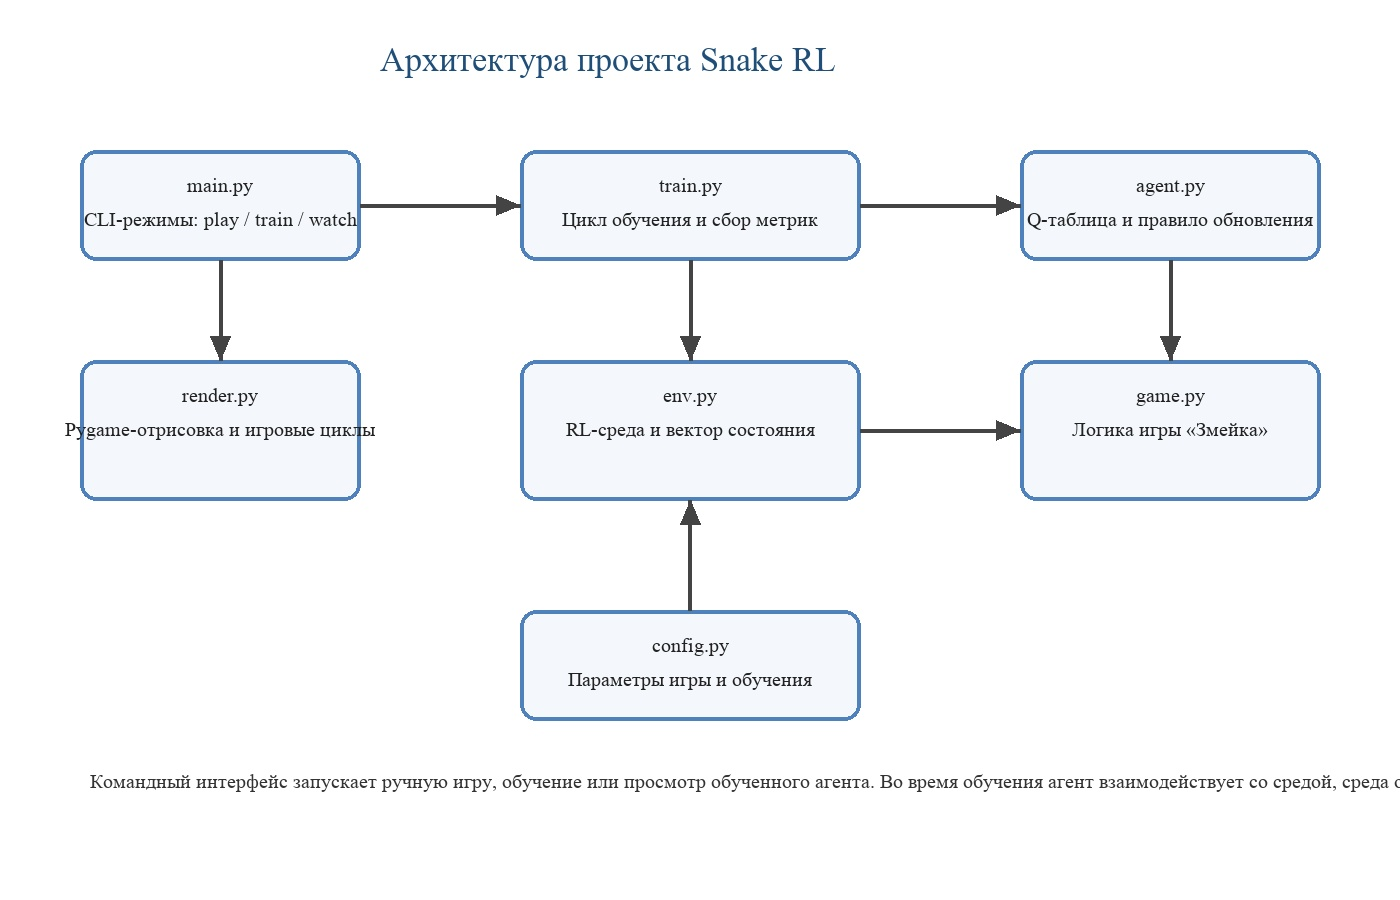
\includegraphics[width=0.80\textwidth]{architecture.jpg}
\end{frame}

% ═══════════════════════════════════════════════════════════════
%  SLIDE 7 — Q-learning
% ═══════════════════════════════════════════════════════════════
\begin{frame}{Алгоритм Q-learning}

\centering
\cardboxc{0.82\textwidth}{%
  \vspace{2pt}
  {\Large $Q(s,a) \;\leftarrow\; Q(s,a) + \alpha\bigl[\,r + \gamma\,\max_{a'}Q(s',a') - Q(s,a)\,\bigr]$}
  \vspace{2pt}
}

\vspace{0.4cm}
\centering
\textcolor{textsub}{\footnotesize ГИПЕРПАРАМЕТРЫ}\\[6pt]
\renewcommand{\arraystretch}{1.3}
\begin{tabular}{cccc}
    \arrayrulecolor{ruleclr}
    \toprule
    $\alpha$ & $\gamma$ & $\varepsilon_{0}$ & decay \\
    \midrule
    \textbf{0.1} & \textbf{0.9} & \textbf{1.0} & \textbf{0.995} \\
    \bottomrule
\end{tabular}
\renewcommand{\arraystretch}{1.0}

\vspace{0.3cm}
$\varepsilon$-жадная стратегия:\quad
\accenttag{$\varepsilon\colon$ 1.0\,$\rightarrow$\,0.05}\quad
{\small--- баланс исследования и использования}
\end{frame}

% ═══════════════════════════════════════════════════════════════
%  SLIDE 8 — Interface
% ═══════════════════════════════════════════════════════════════
\begin{frame}{Интерфейс программы}

\centering
\begin{columns}[c]
\column{0.30\textwidth}
\centering
\begin{tikzpicture}
  \node[inner sep=2pt, draw=ruleclr, rounded corners=6pt,
        blur shadow={shadow blur steps=5,shadow yshift=-1pt,
                     shadow blur radius=2pt}]
    {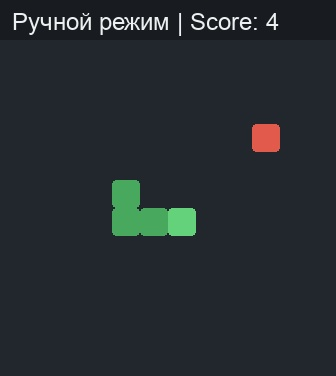
\includegraphics[width=0.92\textwidth]{manual_game.jpg}};
\end{tikzpicture}\\[4pt]
\textcolor{textsub}{\small Ручная игра}

\column{0.30\textwidth}
\centering
\begin{tikzpicture}
  \node[inner sep=2pt, draw=ruleclr, rounded corners=6pt,
        blur shadow={shadow blur steps=5,shadow yshift=-1pt,
                     shadow blur radius=2pt}]
    {
\includegraphics[width=0.92\textwidth]{agent_mode.jpg}};
\end{tikzpicture}\\[4pt]
\textcolor{textsub}{\small Режим агента}

\column{0.30\textwidth}
\centering
\begin{tikzpicture}
  \node[inner sep=2pt, draw=ruleclr, rounded corners=6pt,
        blur shadow={shadow blur steps=5,shadow yshift=-1pt,
                     shadow blur radius=2pt}]
    {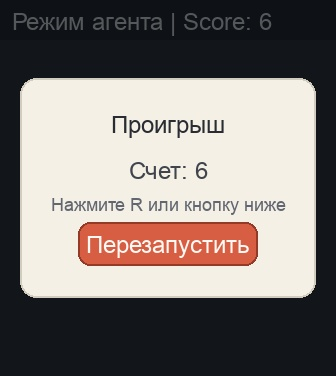
\includegraphics[width=0.92\textwidth]{game_over_modal.jpg}};
\end{tikzpicture}\\[4pt]
\textcolor{textsub}{\small Game over}
\end{columns}
\end{frame}

% ═══════════════════════════════════════════════════════════════
%  SLIDE 9 — Experiment Setup
% ═══════════════════════════════════════════════════════════════
\begin{frame}{Методика эксперимента}

\centering\vspace{0.1cm}
\begin{tikzpicture}[
    nbox/.style={rounded corners=8pt, fill=accentlight, draw=accent!30,
                 minimum width=2.6cm, minimum height=1.4cm,
                 font=\normalsize, text=textmain, align=center,
                 blur shadow={shadow blur steps=5,shadow yshift=-1pt,
                              shadow blur radius=1.5pt}},
  ]
  \node[nbox] (s1) at (0,0)    {\textbf{5}\\[-2pt]{\scriptsize запусков}};
  \node[font=\normalsize,text=accent] at (2.1,0) {$\times$};
  \node[nbox] (s2) at (4.2,0)  {\textbf{8}\\[-2pt]{\scriptsize вариантов}};
  \node[font=\normalsize,text=accent] at (6.3,0) {$\times$};
  \node[nbox] (s3) at (8.4,0)  {\textbf{100}\\[-2pt]{\scriptsize тестов}};
\end{tikzpicture}

\vspace{0.45cm}
\begin{columns}[T]
\column{0.44\textwidth}
\textcolor{textsub}{\footnotesize ЭПИЗОДЫ ОБУЧЕНИЯ}\\[4pt]
50, 100, 200, 300, 500, 800, 1000, 1200

\column{0.44\textwidth}
\textcolor{textsub}{\footnotesize МЕТРИКА}\\[4pt]
Средний score на 100 тестовых играх\\(без исследования, $\varepsilon=0$)
\end{columns}
\end{frame}

% ═══════════════════════════════════════════════════════════════
%  SLIDE 10 — Results Chart
% ═══════════════════════════════════════════════════════════════
\begin{frame}{Результаты обучения}
\centering
\begin{tikzpicture}
  \node[inner sep=4pt, draw=ruleclr, rounded corners=8pt,
        blur shadow={shadow blur steps=5,shadow yshift=-1pt,
                     shadow blur radius=2pt}]
    {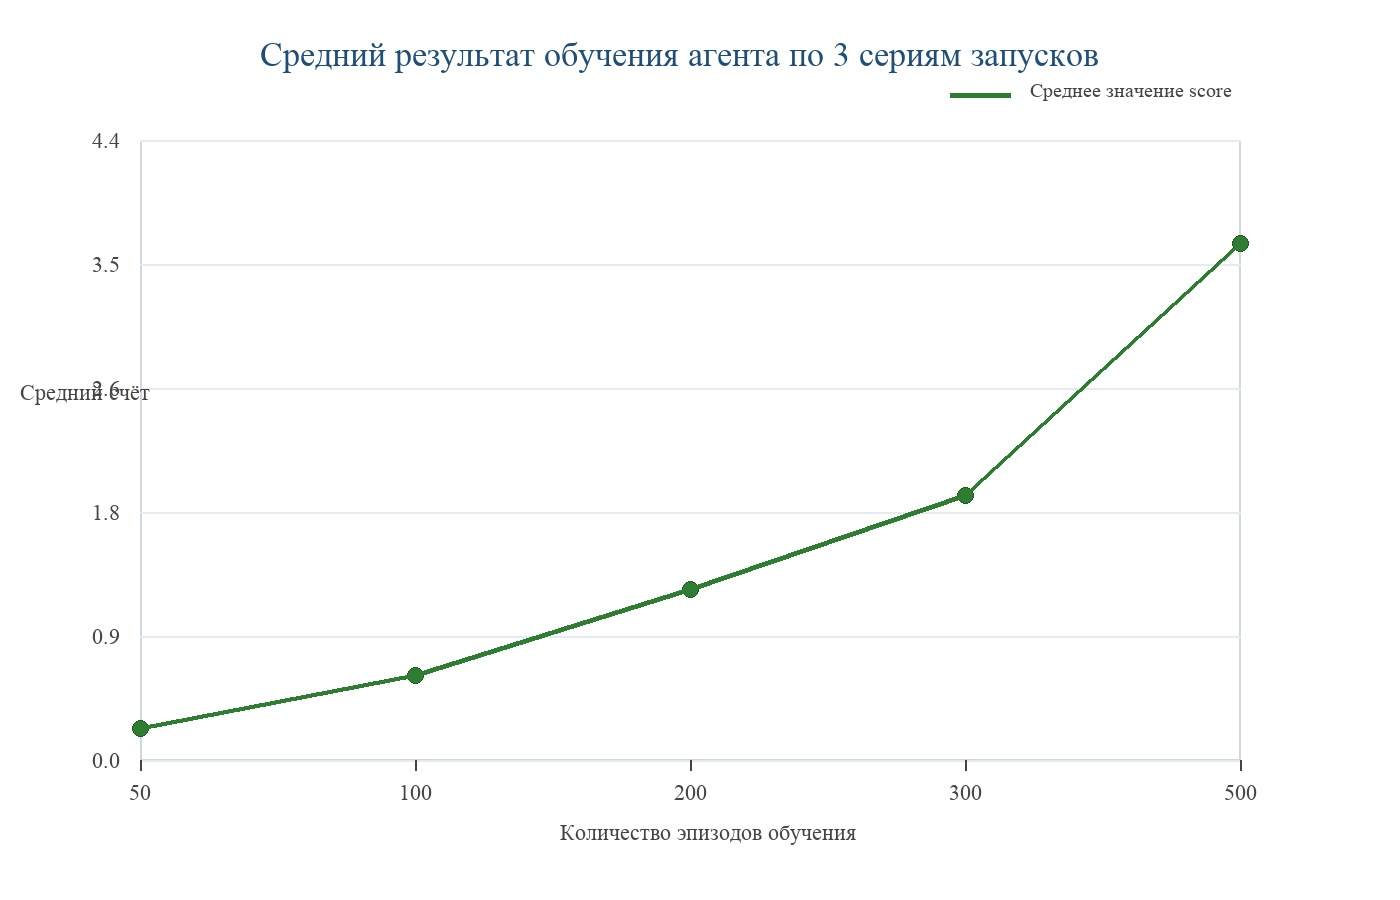
\includegraphics[width=0.76\textwidth]{learning_chart.jpg}};
\end{tikzpicture}
\end{frame}

% ═══════════════════════════════════════════════════════════════
%  SLIDE 11 — Results Table
% ═══════════════════════════════════════════════════════════════
\begin{frame}{Рост качества игры}

\centering
\renewcommand{\arraystretch}{1.5}
\begin{tabular}{ccc}
    \arrayrulecolor{ruleclr}
    \toprule
    \textcolor{textsub}{\footnotesize Эпизоды}
      & \textcolor{textsub}{\footnotesize Средний score}
      & \textcolor{textsub}{\footnotesize Лучший score} \\
    \midrule
    50   & 4.26  & 15.80 \\
    100  & 7.54  & 19.20 \\
    500  & 13.96 & 21.40 \\
    \rowcolor{accentlight}
    1200 & \textbf{16.23} & \textbf{21.60} \\
    \bottomrule
\end{tabular}
\renewcommand{\arraystretch}{1.0}

\vspace{0.35cm}
\begin{columns}[c]
\column{0.44\textwidth}\centering
\cardboxc{0.85\linewidth}{%
  {\footnotesize Средний score}\\[3pt]
  {\Large\textcolor{accentdark}{\textbf{4.26}}%
   \quad{\normalsize$\rightarrow$}\quad%
   \textcolor{accentdark}{\textbf{16.23}}}%
}

\column{0.44\textwidth}\centering
{\small После 800 эпизодов рост замедляется $\Rightarrow$ выход на плато}
\end{columns}
\end{frame}

% ═══════════════════════════════════════════════════════════════
%  SLIDE 12 — Conclusions
% ═══════════════════════════════════════════════════════════════
\begin{frame}{Выводы}

\vspace{0.1cm}
\begin{itemize}\setlength\itemsep{0.35cm}
    \item[\textcolor{greenclr}{\tikz[baseline=-0.6ex]{\fill[greenclr](0,0)circle(1.8pt);}}]
      Цель достигнута: игра реализована, агент обучен, результаты проанализированы
    \item[\textcolor{greenclr}{\tikz[baseline=-0.6ex]{\fill[greenclr](0,0)circle(1.8pt);}}]
      Табличный Q-learning формирует эффективную стратегию без нейросетей
    \item[\textcolor{greenclr}{\tikz[baseline=-0.6ex]{\fill[greenclr](0,0)circle(1.8pt);}}]
      11 бинарных признаков --- компромисс между простотой и информативностью
    \item[\textcolor{accent}{\tikz[baseline=-0.6ex]{\fill[accent](0,0)circle(1.8pt);}}]
      Перспективы: влияние гиперпараметров, DQN для сложных состояний
\end{itemize}

\vspace{0.5cm}
\centering
\begin{tikzpicture}
  \node[fill=accentlight, rounded corners=6pt, inner sep=10pt,
        font=\normalsize, text=accentdark,
        blur shadow={shadow blur steps=5,shadow yshift=-1pt,
                     shadow blur radius=2pt}]
    {Спасибо за внимание};
\end{tikzpicture}
\end{frame}

\end{document}